
\section{Nuclear and Particle}
nuclear properties, radioactive decay, fission
and fusion, reactions, fundamental
properties of elementary particles



\subsection{Light and matter interaction} 
\center
\begin{tabular}{|c|c|}
\hline

Scattering Cross Section & \begin{minipage}{.7 \textwidth}
\small

$\sigma = \dfrac{\mu}{n} = \dfrac{1}{n\Phi}\Big(- \dfrac{d\Phi}{dz}\Big) = \dfrac{1}{nIA}\dfrac{dW}{dz} = \dfrac{P}{\rho l}$, where 

$\sigma$ is the cross section of the event (m$^2$);  

$\mu$ is the attenuation coefficient due to the occurrence of this event (m$^{-1}$); $n$ is the number density of the target particles (m$^{-3}$);

$\Phi$ is the flux of the incident beam;

$-d\Phi$ is the amount of flux lost due to the occurrence of the event (i.e. amount scattered);

$dz$ is the thickness of the target material;

$I$ is the particle flux(or intensity) of the incident beam (m$^{-2}$s$^{-1}$);

$A$ is the area of overlap between beam and target (m$^2$);

$dW$ is the rate at which the event occurs (s$^{-1}$);

$P$ is the probability that a beam particle is scattered;

$\rho$ is the number density ($N/V$) of target particles;

$l$ is the length of the sample (i.e. same as $dz$).

\textbf{If a scattering question is asked, you can probably use dimensional analysis assuming linear relations.}
\end{minipage}

\\ \hline
\end{tabular}


\begin{tabular}{|c|c|}
\hline
\begin{minipage}{.3\textwidth}
Energy ranking of the four major light/matter interactions
\end{minipage}

&
\begin{minipage}{.6\textwidth}

(low energy) Photoelectric $\rightarrow$ Thomson $\rightarrow$ Compton $\rightarrow$ Pair production (high energy)
\end{minipage}

\\ \hline
\end{tabular}
\flushleft

%%%%%%%%%%%%%%%%%%%%%%%%%%%%%%%%%%%%%%%%

\subsection{Particles}

\MiniPg{1}{

\GraphicWHN{.8}{.6}{whatparticle.png}
\tiny .
}

\Table{
\hline

Bosons, Hadrons, Fermions

&

\begin{minipage}{.5\textwidth}
      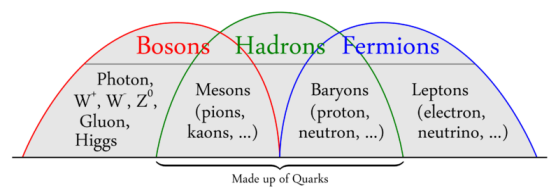
\includegraphics[width=\linewidth, height=30mm]{images/Bosons-Hadrons-Fermions.png}
       \tiny \url{https://commons.wikimedia.org/wiki/File:Bosons-Hadrons-Fermions-RGB-png2.png}

    \end{minipage}

\\ \hline
}

%%%%

\Table{
\hline

The Standard Model & \begin{minipage}{.5\textwidth}
      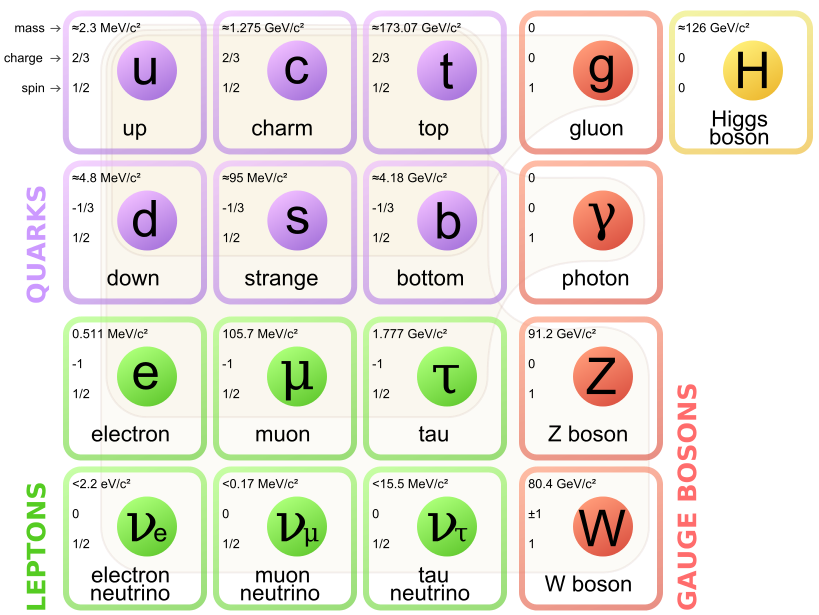
\includegraphics[width=\linewidth, height=60mm]{images/StdMod.png}
       \tiny \url{https://en.wikipedia.org/wiki/Standard_Model}

    \end{minipage}
\\ \hline
}

%%%%

\Table{
\hline

Protium & $^1H$

\\ \hline

Deuterium & 
\begin{minipage}{0.6 \textwidth}

Symbol: D or $^2$H. Also known as `heavy hydrogen'. Nucleus consists of one proton and one neutron.

\end{minipage}

\\ \hline
}

%%%%

\Table{
\hline

Deuteron & 
\begin{minipage}{0.6 \textwidth}
The nucleus of deuterium. It is a boson and exists in the triplet state. The singlet state is virtual and only transiently exists during neutron-proton inelastic scattering. Duh!

\end{minipage}

\\ \hline
}

%%%%

\Table{
\hline

Tritium &
\begin{minipage}{0.6 \textwidth}

T or $^3$H. One proton, two neutrons. Watch out.

\end{minipage}

\\ \hline

Triton & Yup. You guessed it.

\\ \hline
}

%%%%%%%%%%%%%%%%%%%%%%%%%%%%%%%%%%

\subsection{Nuclear properties}
\Table{
\hline

\MiniPg{.25}{
Nuclear binding energy
}
&
\begin{minipage}{.75\textwidth}
      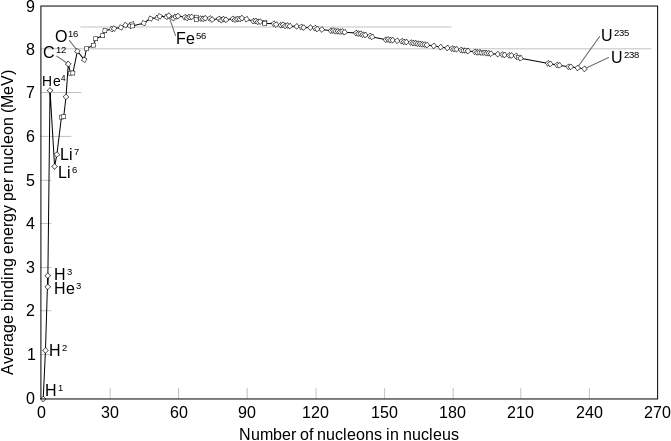
\includegraphics[width=\linewidth, height=60mm]{images/NucBindingEn.png}
      
      \small
      
    \textbf{H to Na} -  increasing ``forces per nucleon in the nucleus, as each additional nucleon is attracted by other nearby nucleons, and thus more tightly bound to the whole.";
   \textbf{Mg to Xe} (``saturation") - ``the nucleus has become large enough that nuclear forces no longer completely extend efficiently across its width. Attractive nuclear forces in this region, as atomic mass increases, are nearly balanced by repellent electromagnetic forces between protons, as the atomic number increases.";
   \textbf{Cs to U} - ``electromagnetic repulsive forces are beginning to overcome the strong nuclear force attraction."
   
   \tiny \url{https://en.wikipedia.org/wiki/Nuclear_binding_energy}
    \end{minipage}
 
 \\ \hline
}

%%%%%%%%%%%%%%%%%%%%%%%%%%%%%%%%%%%%%%%
\subsection{Radioactive decay} 
\Table{
\hline
\MiniPg{.3}{
Alpha decay, beta decay, gamma decay, positron emission, electron capture
}

&

\MiniPg{.7}{

\GraphicWHN{1}{.7}{RadioDecay.png}

\tiny \url{http://chemwiki.ucdavis.edu/Textbook_Maps/General_Chemistry_Textbook_Maps/Map\%3A_Chemistry_(OpenSTAX)/21\%3A_Nuclear_Chemistry/21.3\%3A_Radioactive_Decay}

}

\\ \hline
}
%%%%%%%%%%%%%%%%%%%%%%%%%%%%%%%%%%%%%%%

\subsection{Fission and fusion} 
\Table{
\hline
Deuterium tritium fusion

&

\MiniPg{.6}{
\GraphicWHN{.5}{.5}{DeutTritFusion.png}
\tiny \url{https://en.wikipedia.org/wiki/Nuclear_fusion}
}
 
 \\ \hline
}

%%%%
\Table{
\hline

Deuterium Deuterium fusion

 &
 
\MiniPg{.6}{
\GraphicWHN{.9}{.6}{DeutDeutFusion.jpg}
\tiny \url{http://resource.download.wjec.co.uk/vtc/2008-09/science/irf08_48/Images/Nuclear-fusion.jpg}

}
 
 \\ \hline
}

%%%%

\Table{
\hline
\MiniPg{.4}{\center
Proton Proton chain fusion reaction in the sun and smaller stars
}

&

\MiniPg{.6}{\center

\GraphicWHN{.4}{.6}{FusionintheSun.png}
\tiny \url{https://en.wikipedia.org/wiki/Nuclear_fusion}
}

\\ \hline
}

%%%%%%%%%%%%%%%%%%%%%%%%%%%%

\subsection{Reactions} 
\center
\begin{tabular}{|c|c|}
\hline

Chemical symbol convention & $^{A}_{Z}Na^{C} $ \\
& where $A = $ Mass \# of protons $+$ neutrons, \\
& $Z =$ Atomic \# of protons, \\
& $C = $ Charge, e.g. '$+2$'
 
 \\ \hline
\end{tabular}
\flushleft

%%%%%%%%%%%%%%%%%%%%%%%%%%%%%%%%%%%%%%%%

\subsection{Fundamental properties of elementary particles} 


